% Options for packages loaded elsewhere
\PassOptionsToPackage{unicode}{hyperref}
\PassOptionsToPackage{hyphens}{url}
%
\documentclass[
]{article}
\usepackage{lmodern}
\usepackage{amssymb,amsmath}
\usepackage{ifxetex,ifluatex}
\ifnum 0\ifxetex 1\fi\ifluatex 1\fi=0 % if pdftex
  \usepackage[T1]{fontenc}
  \usepackage[utf8]{inputenc}
  \usepackage{textcomp} % provide euro and other symbols
\else % if luatex or xetex
  \usepackage{unicode-math}
  \defaultfontfeatures{Scale=MatchLowercase}
  \defaultfontfeatures[\rmfamily]{Ligatures=TeX,Scale=1}
\fi
% Use upquote if available, for straight quotes in verbatim environments
\IfFileExists{upquote.sty}{\usepackage{upquote}}{}
\IfFileExists{microtype.sty}{% use microtype if available
  \usepackage[]{microtype}
  \UseMicrotypeSet[protrusion]{basicmath} % disable protrusion for tt fonts
}{}
\makeatletter
\@ifundefined{KOMAClassName}{% if non-KOMA class
  \IfFileExists{parskip.sty}{%
    \usepackage{parskip}
  }{% else
    \setlength{\parindent}{0pt}
    \setlength{\parskip}{6pt plus 2pt minus 1pt}}
}{% if KOMA class
  \KOMAoptions{parskip=half}}
\makeatother
\usepackage{xcolor}
\IfFileExists{xurl.sty}{\usepackage{xurl}}{} % add URL line breaks if available
\IfFileExists{bookmark.sty}{\usepackage{bookmark}}{\usepackage{hyperref}}
\hypersetup{
  pdftitle={Course Project 1},
  pdfauthor={Eduardo HeCo},
  hidelinks,
  pdfcreator={LaTeX via pandoc}}
\urlstyle{same} % disable monospaced font for URLs
\usepackage[margin=1in]{geometry}
\usepackage{color}
\usepackage{fancyvrb}
\newcommand{\VerbBar}{|}
\newcommand{\VERB}{\Verb[commandchars=\\\{\}]}
\DefineVerbatimEnvironment{Highlighting}{Verbatim}{commandchars=\\\{\}}
% Add ',fontsize=\small' for more characters per line
\usepackage{framed}
\definecolor{shadecolor}{RGB}{248,248,248}
\newenvironment{Shaded}{\begin{snugshade}}{\end{snugshade}}
\newcommand{\AlertTok}[1]{\textcolor[rgb]{0.94,0.16,0.16}{#1}}
\newcommand{\AnnotationTok}[1]{\textcolor[rgb]{0.56,0.35,0.01}{\textbf{\textit{#1}}}}
\newcommand{\AttributeTok}[1]{\textcolor[rgb]{0.77,0.63,0.00}{#1}}
\newcommand{\BaseNTok}[1]{\textcolor[rgb]{0.00,0.00,0.81}{#1}}
\newcommand{\BuiltInTok}[1]{#1}
\newcommand{\CharTok}[1]{\textcolor[rgb]{0.31,0.60,0.02}{#1}}
\newcommand{\CommentTok}[1]{\textcolor[rgb]{0.56,0.35,0.01}{\textit{#1}}}
\newcommand{\CommentVarTok}[1]{\textcolor[rgb]{0.56,0.35,0.01}{\textbf{\textit{#1}}}}
\newcommand{\ConstantTok}[1]{\textcolor[rgb]{0.00,0.00,0.00}{#1}}
\newcommand{\ControlFlowTok}[1]{\textcolor[rgb]{0.13,0.29,0.53}{\textbf{#1}}}
\newcommand{\DataTypeTok}[1]{\textcolor[rgb]{0.13,0.29,0.53}{#1}}
\newcommand{\DecValTok}[1]{\textcolor[rgb]{0.00,0.00,0.81}{#1}}
\newcommand{\DocumentationTok}[1]{\textcolor[rgb]{0.56,0.35,0.01}{\textbf{\textit{#1}}}}
\newcommand{\ErrorTok}[1]{\textcolor[rgb]{0.64,0.00,0.00}{\textbf{#1}}}
\newcommand{\ExtensionTok}[1]{#1}
\newcommand{\FloatTok}[1]{\textcolor[rgb]{0.00,0.00,0.81}{#1}}
\newcommand{\FunctionTok}[1]{\textcolor[rgb]{0.00,0.00,0.00}{#1}}
\newcommand{\ImportTok}[1]{#1}
\newcommand{\InformationTok}[1]{\textcolor[rgb]{0.56,0.35,0.01}{\textbf{\textit{#1}}}}
\newcommand{\KeywordTok}[1]{\textcolor[rgb]{0.13,0.29,0.53}{\textbf{#1}}}
\newcommand{\NormalTok}[1]{#1}
\newcommand{\OperatorTok}[1]{\textcolor[rgb]{0.81,0.36,0.00}{\textbf{#1}}}
\newcommand{\OtherTok}[1]{\textcolor[rgb]{0.56,0.35,0.01}{#1}}
\newcommand{\PreprocessorTok}[1]{\textcolor[rgb]{0.56,0.35,0.01}{\textit{#1}}}
\newcommand{\RegionMarkerTok}[1]{#1}
\newcommand{\SpecialCharTok}[1]{\textcolor[rgb]{0.00,0.00,0.00}{#1}}
\newcommand{\SpecialStringTok}[1]{\textcolor[rgb]{0.31,0.60,0.02}{#1}}
\newcommand{\StringTok}[1]{\textcolor[rgb]{0.31,0.60,0.02}{#1}}
\newcommand{\VariableTok}[1]{\textcolor[rgb]{0.00,0.00,0.00}{#1}}
\newcommand{\VerbatimStringTok}[1]{\textcolor[rgb]{0.31,0.60,0.02}{#1}}
\newcommand{\WarningTok}[1]{\textcolor[rgb]{0.56,0.35,0.01}{\textbf{\textit{#1}}}}
\usepackage{graphicx,grffile}
\makeatletter
\def\maxwidth{\ifdim\Gin@nat@width>\linewidth\linewidth\else\Gin@nat@width\fi}
\def\maxheight{\ifdim\Gin@nat@height>\textheight\textheight\else\Gin@nat@height\fi}
\makeatother
% Scale images if necessary, so that they will not overflow the page
% margins by default, and it is still possible to overwrite the defaults
% using explicit options in \includegraphics[width, height, ...]{}
\setkeys{Gin}{width=\maxwidth,height=\maxheight,keepaspectratio}
% Set default figure placement to htbp
\makeatletter
\def\fps@figure{htbp}
\makeatother
\setlength{\emergencystretch}{3em} % prevent overfull lines
\providecommand{\tightlist}{%
  \setlength{\itemsep}{0pt}\setlength{\parskip}{0pt}}
\setcounter{secnumdepth}{-\maxdimen} % remove section numbering

\title{Course Project 1}
\author{Eduardo HeCo}
\date{16/8/2020}

\begin{document}
\maketitle

\#Download the data

\begin{Shaded}
\begin{Highlighting}[]
\KeywordTok{library}\NormalTok{(}\StringTok{"data.table"}\NormalTok{)}
\end{Highlighting}
\end{Shaded}

\begin{verbatim}
## Warning: package 'data.table' was built under R version 3.6.3
\end{verbatim}

\begin{Shaded}
\begin{Highlighting}[]
\NormalTok{Url<-}\StringTok{"https://d396qusza40orc.cloudfront.net/repdata%2Fdata%2Factivity.zip"}
\KeywordTok{download.file}\NormalTok{(Url,}\DataTypeTok{destfile=}\KeywordTok{paste0}\NormalTok{(}\KeywordTok{getwd}\NormalTok{(), }\StringTok{'/repdata%2Fdata%2Factivity.zip'}\NormalTok{),}\DataTypeTok{method=}\StringTok{"curl"}\NormalTok{)}
\KeywordTok{unzip}\NormalTok{(}\StringTok{"repdata%2Fdata%2Factivity.zip"}\NormalTok{,}\DataTypeTok{exdir=}\StringTok{"data"}\NormalTok{)}
\end{Highlighting}
\end{Shaded}

\#Reading the data

\begin{Shaded}
\begin{Highlighting}[]
\NormalTok{Datos<-}\KeywordTok{read.csv}\NormalTok{(}\StringTok{"activity.csv"}\NormalTok{)}
\NormalTok{DatosNA<-Datos[}\OperatorTok{!}\KeywordTok{is.na}\NormalTok{(Datos}\OperatorTok{$}\NormalTok{steps),]}
\end{Highlighting}
\end{Shaded}

\#What is mean total number of steps taken per day? \#1.Calculate the
total number of steps taken per day

\begin{Shaded}
\begin{Highlighting}[]
\NormalTok{numberofsteps<-}\KeywordTok{tapply}\NormalTok{(DatosNA}\OperatorTok{$}\NormalTok{steps,DatosNA}\OperatorTok{$}\NormalTok{date,mean)}
\KeywordTok{as.data.frame}\NormalTok{(numberofsteps)}
\end{Highlighting}
\end{Shaded}

\begin{verbatim}
##            numberofsteps
## 2012-10-01            NA
## 2012-10-02     0.4375000
## 2012-10-03    39.4166667
## 2012-10-04    42.0694444
## 2012-10-05    46.1597222
## 2012-10-06    53.5416667
## 2012-10-07    38.2465278
## 2012-10-08            NA
## 2012-10-09    44.4826389
## 2012-10-10    34.3750000
## 2012-10-11    35.7777778
## 2012-10-12    60.3541667
## 2012-10-13    43.1458333
## 2012-10-14    52.4236111
## 2012-10-15    35.2048611
## 2012-10-16    52.3750000
## 2012-10-17    46.7083333
## 2012-10-18    34.9166667
## 2012-10-19    41.0729167
## 2012-10-20    36.0937500
## 2012-10-21    30.6284722
## 2012-10-22    46.7361111
## 2012-10-23    30.9652778
## 2012-10-24    29.0104167
## 2012-10-25     8.6527778
## 2012-10-26    23.5347222
## 2012-10-27    35.1354167
## 2012-10-28    39.7847222
## 2012-10-29    17.4236111
## 2012-10-30    34.0937500
## 2012-10-31    53.5208333
## 2012-11-01            NA
## 2012-11-02    36.8055556
## 2012-11-03    36.7048611
## 2012-11-04            NA
## 2012-11-05    36.2465278
## 2012-11-06    28.9375000
## 2012-11-07    44.7326389
## 2012-11-08    11.1770833
## 2012-11-09            NA
## 2012-11-10            NA
## 2012-11-11    43.7777778
## 2012-11-12    37.3784722
## 2012-11-13    25.4722222
## 2012-11-14            NA
## 2012-11-15     0.1423611
## 2012-11-16    18.8923611
## 2012-11-17    49.7881944
## 2012-11-18    52.4652778
## 2012-11-19    30.6979167
## 2012-11-20    15.5277778
## 2012-11-21    44.3993056
## 2012-11-22    70.9270833
## 2012-11-23    73.5902778
## 2012-11-24    50.2708333
## 2012-11-25    41.0902778
## 2012-11-26    38.7569444
## 2012-11-27    47.3819444
## 2012-11-28    35.3576389
## 2012-11-29    24.4687500
## 2012-11-30            NA
\end{verbatim}

\#2. If you do not understand the difference between a histogram \#and a
barplot, research the difference between them. \#Make a histogram of the
total number of steps taken each day.

\begin{Shaded}
\begin{Highlighting}[]
\KeywordTok{library}\NormalTok{(lattice)}
\KeywordTok{histogram}\NormalTok{(numberofsteps,}\DataTypeTok{col=}\StringTok{"lightblue"}\NormalTok{,}\DataTypeTok{xlab=}\StringTok{"Total number of steps taken each day"}\NormalTok{,}\DataTypeTok{main=}\StringTok{"Histogram of total steps by day"}\NormalTok{)}
\end{Highlighting}
\end{Shaded}

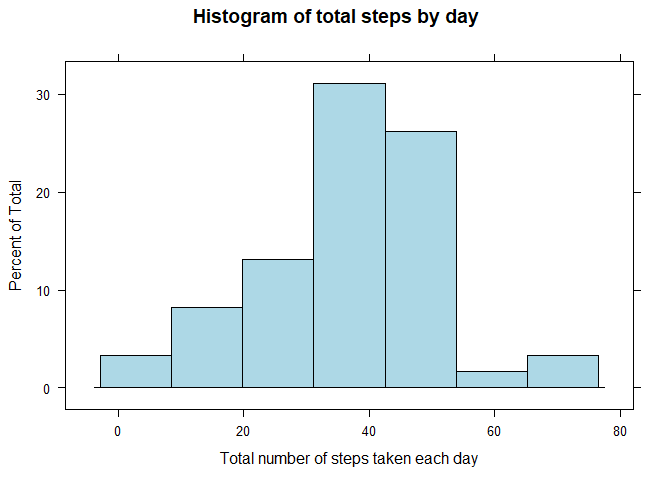
\includegraphics{PA1_templates_files/figure-latex/histogram-1.pdf} \#3
Calculate and report the mean and median of the total number of \#steps
taken per day

\begin{Shaded}
\begin{Highlighting}[]
\KeywordTok{tapply}\NormalTok{(DatosNA}\OperatorTok{$}\NormalTok{steps,DatosNA}\OperatorTok{$}\NormalTok{date,mean)->meannumsteps}
\KeywordTok{tapply}\NormalTok{(DatosNA}\OperatorTok{$}\NormalTok{steps,DatosNA}\OperatorTok{$}\NormalTok{date,median)->mediannumsteps}
\end{Highlighting}
\end{Shaded}

\#What is the average daily activity pattern? \#1. Make a time series
plot (i.e.~\color{red}{\verb|type = "l"|}type = ``l'') of the 5-minute
interval (x-axis) and the average number of steps taken, averaged across
all days (y-axis)

\begin{Shaded}
\begin{Highlighting}[]
\NormalTok{DatosNA}\OperatorTok{$}\NormalTok{steps<-}\KeywordTok{na.omit}\NormalTok{(DatosNA}\OperatorTok{$}\NormalTok{steps)}
\KeywordTok{tapply}\NormalTok{(DatosNA}\OperatorTok{$}\NormalTok{steps,DatosNA}\OperatorTok{$}\NormalTok{interval,mean)->meantepsbyinterval}
\KeywordTok{plot}\NormalTok{(meantepsbyinterval,}\DataTypeTok{type=}\StringTok{"l"}\NormalTok{,}\DataTypeTok{xlab=}\StringTok{"Intervals per day"}\NormalTok{,}\DataTypeTok{ylab=}\StringTok{"Average steps"}\NormalTok{)}
\end{Highlighting}
\end{Shaded}

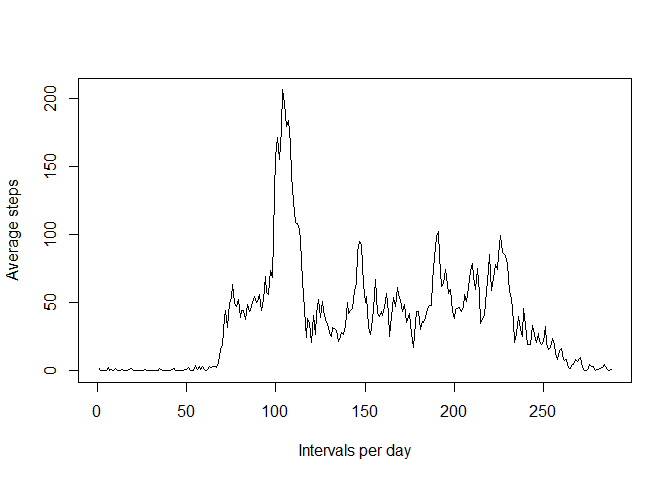
\includegraphics{PA1_templates_files/figure-latex/unnamed-chunk-1-1.pdf}
\#2. Which 5-minute interval, on average across all the days in the
dataset, contains the maximum number of steps?

\begin{Shaded}
\begin{Highlighting}[]
\NormalTok{summ<-}\KeywordTok{max}\NormalTok{(meantepsbyinterval)}
\KeywordTok{which}\NormalTok{(meantepsbyinterval}\OperatorTok{==}\NormalTok{summ)}
\end{Highlighting}
\end{Shaded}

\begin{verbatim}
## 835 
## 104
\end{verbatim}

\#Imputing missing values \#1.Calculate and report the total number of
missing values in the dataset (i.e.~the total number of rows with NAs)

\begin{verbatim}
sum(is.na(Datos))
\end{verbatim}

\#Devise a strategy for filling in all of the missing values in the
dataset. The strategy does not need to be sophisticated. For example,
you could use the mean/median for that day, or the mean for that
5-minute interval, etc.

\begin{Shaded}
\begin{Highlighting}[]
\KeywordTok{print}\NormalTok{(}\StringTok{"The the values of the missing values were filled with the mean of 5-minute interval"}\NormalTok{)}
\end{Highlighting}
\end{Shaded}

\begin{verbatim}
## [1] "The the values of the missing values were filled with the mean of 5-minute interval"
\end{verbatim}

\#Create a new dataset that is equal to the original dataset but with
the missing data filled in.

\begin{Shaded}
\begin{Highlighting}[]
\KeywordTok{as.data.frame}\NormalTok{(meantepsbyinterval)->meantepsbyinterval}
\NormalTok{InterVal<-}\KeywordTok{head}\NormalTok{(Datos}\OperatorTok{$}\NormalTok{interval,}\DecValTok{288}\NormalTok{)}
\NormalTok{meantepsbyinterval<-}\KeywordTok{cbind}\NormalTok{(InterVal,meantepsbyinterval)}
\KeywordTok{colnames}\NormalTok{(meantepsbyinterval)<-}\KeywordTok{c}\NormalTok{(}\StringTok{"min"}\NormalTok{,}\StringTok{"means"}\NormalTok{)}
\NormalTok{dataNA<-}\ControlFlowTok{function}\NormalTok{(Datos,meantepsbyinterval)}
\NormalTok{\{}
\NormalTok{  DataNAs<-Datos}
    \ControlFlowTok{for}\NormalTok{(i }\ControlFlowTok{in} \DecValTok{1}\OperatorTok{:}\KeywordTok{nrow}\NormalTok{(DataNAs))}
\NormalTok{    \{}
       \ControlFlowTok{if}\NormalTok{(}\KeywordTok{is.na}\NormalTok{(DataNAs[i,}\StringTok{"steps"}\NormalTok{]))}
\NormalTok{       \{}
\NormalTok{          interval<-DataNAs[i,}\StringTok{"interval"}\NormalTok{]}
\NormalTok{          DataNAs[i,}\StringTok{"steps"}\NormalTok{]=meantepsbyinterval[}\KeywordTok{which}\NormalTok{(meantepsbyinterval}\OperatorTok{$}\NormalTok{min}\OperatorTok{==}\NormalTok{interval),}\StringTok{"means"}\NormalTok{]}
\NormalTok{       \}}
\NormalTok{    \}}
\NormalTok{DataNAs}
\NormalTok{\}}
\NormalTok{dataNAs<-}\KeywordTok{dataNA}\NormalTok{(Datos,meantepsbyinterval)}
\end{Highlighting}
\end{Shaded}

\#Make a histogram of the total number of steps taken each day and
Calculate and report the mean and median total number of steps taken per
day. Do these values differ from the estimates from the first part of
the assignment? What is the impact of imputing missing data on the
estimates of the total daily number of steps? \#The impact of imputing
missing data is shown in the graph and you can see how the NA filled
data is more defined.

\begin{Shaded}
\begin{Highlighting}[]
\NormalTok{numberofsteps2<-}\KeywordTok{tapply}\NormalTok{(dataNAs}\OperatorTok{$}\NormalTok{steps,dataNAs}\OperatorTok{$}\NormalTok{date,mean)}
\KeywordTok{histogram}\NormalTok{(numberofsteps2,}\DataTypeTok{col=}\StringTok{"lightblue"}\NormalTok{,}\DataTypeTok{xlab=}\StringTok{"Total number of steps taken each day"}\NormalTok{,}\DataTypeTok{main=}\StringTok{"Histogram of total steps by day"}\NormalTok{)}
\end{Highlighting}
\end{Shaded}

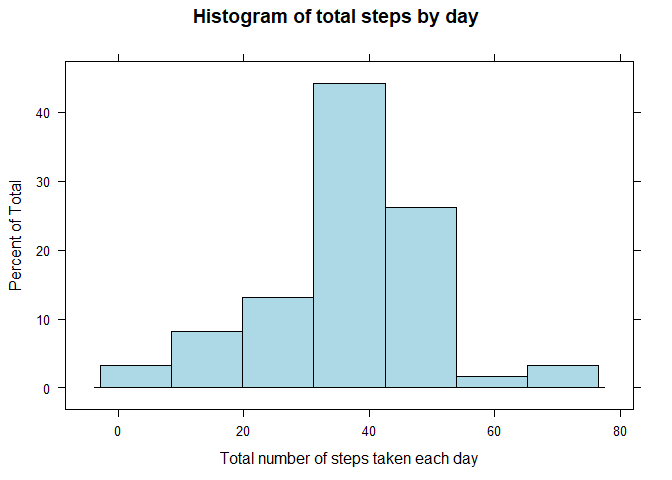
\includegraphics{PA1_templates_files/figure-latex/unnamed-chunk-5-1.pdf}

\begin{Shaded}
\begin{Highlighting}[]
\KeywordTok{tapply}\NormalTok{(dataNAs}\OperatorTok{$}\NormalTok{steps,dataNAs}\OperatorTok{$}\NormalTok{date,mean)->meannumsteps2}
\KeywordTok{tapply}\NormalTok{(dataNAs}\OperatorTok{$}\NormalTok{steps,dataNAs}\OperatorTok{$}\NormalTok{date,median)->mediannumsteps2}
\KeywordTok{tapply}\NormalTok{(dataNAs}\OperatorTok{$}\NormalTok{steps,dataNAs}\OperatorTok{$}\NormalTok{interval,mean)->meantepsbyinterval3}
\KeywordTok{par}\NormalTok{(}\DataTypeTok{mfrow=}\KeywordTok{c}\NormalTok{(}\DecValTok{2}\NormalTok{,}\DecValTok{1}\NormalTok{))}
\KeywordTok{plot}\NormalTok{(meantepsbyinterval,}\DataTypeTok{type=}\StringTok{"l"}\NormalTok{,}\DataTypeTok{xlab=}\StringTok{"Intervals per day"}\NormalTok{,}\DataTypeTok{ylab=}\StringTok{"Average steps"}\NormalTok{,}\DataTypeTok{main=}\StringTok{"Original data"}\NormalTok{)}
\KeywordTok{plot}\NormalTok{(meantepsbyinterval3,}\DataTypeTok{type=}\StringTok{"l"}\NormalTok{,}\DataTypeTok{xlab=}\StringTok{"Intervals per day"}\NormalTok{,}\DataTypeTok{ylab=}\StringTok{"Average steps"}\NormalTok{,}\DataTypeTok{main=}\StringTok{"NA filled data"}\NormalTok{)}
\end{Highlighting}
\end{Shaded}

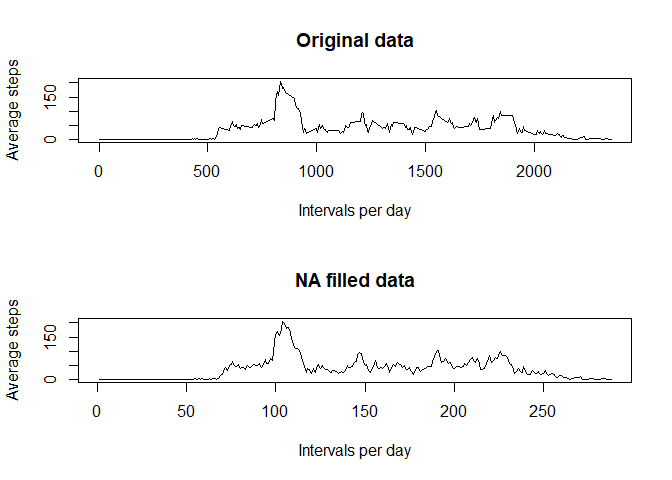
\includegraphics{PA1_templates_files/figure-latex/unnamed-chunk-5-2.pdf}
\#Create a new factor variable in the dataset with two levels --
``weekday'' and ``weekend'' indicating whether a given date is a weekday
or weekend day.

\begin{Shaded}
\begin{Highlighting}[]
\KeywordTok{Sys.setlocale}\NormalTok{(}\StringTok{"LC_TIME"}\NormalTok{, }\StringTok{"English"}\NormalTok{)}
\end{Highlighting}
\end{Shaded}

\begin{verbatim}
## [1] "English_United States.1252"
\end{verbatim}

\begin{Shaded}
\begin{Highlighting}[]
\NormalTok{weekdayss<-}\KeywordTok{c}\NormalTok{(}\StringTok{"Monday"}\NormalTok{,}\StringTok{"Tuesday"}\NormalTok{,}\StringTok{"Wednesday"}\NormalTok{,}\StringTok{"Thursday"}\NormalTok{,}\StringTok{"Friday"}\NormalTok{)}
\NormalTok{dataNAs}\OperatorTok{$}\NormalTok{date<-}\KeywordTok{as.Date}\NormalTok{(dataNAs}\OperatorTok{$}\NormalTok{date)}
\NormalTok{dataNAs}\OperatorTok{$}\NormalTok{weekday<-}\KeywordTok{factor}\NormalTok{((}\KeywordTok{weekdays}\NormalTok{(dataNAs}\OperatorTok{$}\NormalTok{date) }\OperatorTok\StringTok{ }\NormalTok{weekdayss),}\DataTypeTok{levels=}\KeywordTok{c}\NormalTok{(}\OtherTok{FALSE}\NormalTok{,}\OtherTok{TRUE}\NormalTok{),}\DataTypeTok{labels=}\KeywordTok{c}\NormalTok{(}\StringTok{"weekend"}\NormalTok{,}\StringTok{"weekday"}\NormalTok{)) }
\KeywordTok{unique}\NormalTok{(dataNAs}\OperatorTok{$}\NormalTok{weekday)}
\end{Highlighting}
\end{Shaded}

\begin{verbatim}
## [1] weekday weekend
## Levels: weekend weekday
\end{verbatim}

\begin{Shaded}
\begin{Highlighting}[]
\KeywordTok{head}\NormalTok{(dataNAs)}
\end{Highlighting}
\end{Shaded}

\begin{verbatim}
##       steps       date interval weekday
## 1 1.7169811 2012-10-01        0 weekday
## 2 0.3396226 2012-10-01        5 weekday
## 3 0.1320755 2012-10-01       10 weekday
## 4 0.1509434 2012-10-01       15 weekday
## 5 0.0754717 2012-10-01       20 weekday
## 6 2.0943396 2012-10-01       25 weekday
\end{verbatim}

\#Make a panel plot containing a time series plot
(i.e.~\color{red}{\verb|type = "l"|}type = ``l'') of the 5-minute
interval (x-axis) and the average number of steps taken, averaged across
all weekday days or weekend days (y-axis). See the README file in the
GitHub repository to see an example of what this plot should look like
using simulated data.

\begin{Shaded}
\begin{Highlighting}[]
\NormalTok{weekDayDatos<-dataNAs[}\KeywordTok{which}\NormalTok{(dataNAs}\OperatorTok{$}\NormalTok{weekday}\OperatorTok{==}\StringTok{"weekday"}\NormalTok{),]}
\NormalTok{weekendDatos<-dataNAs[}\KeywordTok{which}\NormalTok{(dataNAs}\OperatorTok{$}\NormalTok{weekday}\OperatorTok{==}\StringTok{"weekend"}\NormalTok{),]}
\NormalTok{meanweekday<-}\KeywordTok{tapply}\NormalTok{(weekDayDatos}\OperatorTok{$}\NormalTok{steps,weekDayDatos}\OperatorTok{$}\NormalTok{interval,mean)}
\NormalTok{meanweekend<-}\KeywordTok{tapply}\NormalTok{(weekendDatos}\OperatorTok{$}\NormalTok{steps,weekendDatos}\OperatorTok{$}\NormalTok{interval,mean)}
\KeywordTok{par}\NormalTok{(}\DataTypeTok{mfrow=}\KeywordTok{c}\NormalTok{(}\DecValTok{2}\NormalTok{,}\DecValTok{1}\NormalTok{))}
\KeywordTok{plot}\NormalTok{(meanweekday,}\DataTypeTok{main=}\StringTok{"Weekday"}\NormalTok{,}\DataTypeTok{xlab=}\StringTok{"interval"}\NormalTok{,}\DataTypeTok{ylab=}\StringTok{"Number of steps"}\NormalTok{,}\DataTypeTok{type=}\StringTok{"l"}\NormalTok{)}
\KeywordTok{plot}\NormalTok{(meanweekend,}\DataTypeTok{main=}\StringTok{"Weekend"}\NormalTok{,}\DataTypeTok{xlab=}\StringTok{"interval"}\NormalTok{,}\DataTypeTok{ylab=}\StringTok{"Number of steps"}\NormalTok{,}\DataTypeTok{type=}\StringTok{"l"}\NormalTok{)}
\end{Highlighting}
\end{Shaded}

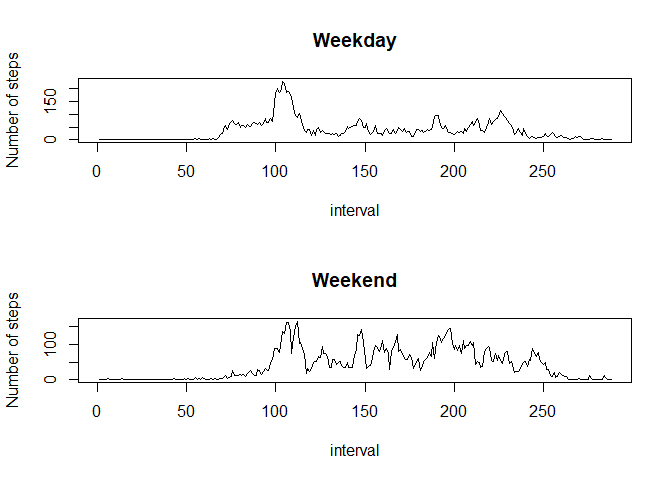
\includegraphics{PA1_templates_files/figure-latex/unnamed-chunk-7-1.pdf}

\hypertarget{r-markdown}{%
\subsection{R Markdown}\label{r-markdown}}

This is an R Markdown document. Markdown is a simple formatting syntax
for authoring HTML, PDF, and MS Word documents. For more details on
using R Markdown see \url{http://rmarkdown.rstudio.com}.

When you click the \textbf{Knit} button a document will be generated
that includes both content as well as the output of any embedded R code
chunks within the document. You can embed an R code chunk like this:

\begin{Shaded}
\begin{Highlighting}[]
\KeywordTok{summary}\NormalTok{(cars)}
\end{Highlighting}
\end{Shaded}

\begin{verbatim}
##      speed           dist       
##  Min.   : 4.0   Min.   :  2.00  
##  1st Qu.:12.0   1st Qu.: 26.00  
##  Median :15.0   Median : 36.00  
##  Mean   :15.4   Mean   : 42.98  
##  3rd Qu.:19.0   3rd Qu.: 56.00  
##  Max.   :25.0   Max.   :120.00
\end{verbatim}

\hypertarget{including-plots}{%
\subsection{Including Plots}\label{including-plots}}

You can also embed plots, for example:

\includegraphics{PA1_templates_files/figure-latex/pressure-1.pdf}

Note that the \texttt{echo\ =\ FALSE} parameter was added to the code
chunk to prevent printing of the R code that generated the plot.

\end{document}
